\section{Objetivo}
\begin{itemize}
    \item Obtener la curva de magnetización del núcleo ferromagnético de un reactor.
    \item Observar en el osciloscopio el lazo de histéresis dinámico y la forma de onda de la corriente de excitación.
    \item Realizar la separación de pérdidas del núcleo.
\end{itemize}

\section{Fundamento teórico}
Transformador monofásico\\
Es un dispositivo eléctrico que permite aumentar o disminuir la tensión en un circuito eléctrico de corriente alterna, manteniendo la frecuencia. Está constituido por dos o más bobinas de material conductor, aisladas entre sí eléctricamente y por lo general enrolladas alrededor de un mismo núcleo de material ferro magnético. La única conexión entre las bobinas la constituye el flujo magnético común que se establece en el núcleo.
\begin{figure}[H]
    \centering
    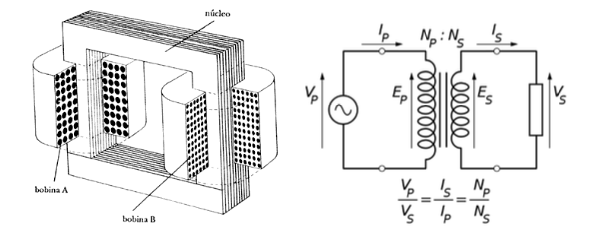
\includegraphics[width=0.7\textwidth]{modelo_equivalente.png}
    \captionsetup{labelformat=empty}
    \caption{Modelo eléctrico equivalente}
\end{figure}

\section{Procedimiento}

\subsection{Obtención de resistencias en D.C.}
Medir las resistencias de cada enrollamiento y anotar la temperatura ambiente. Corregir los valores a la temperatura normalizada de referencia $75C$.

\subsection{Prueba de vacío}
Consiste en aplicar una tensión nominal V1 en cualquiera de los enrollados del transformador, con el otro enrollado abierto, se le aplica al lado 1 voltaje y frecuencia nominal, registrándose las lecturas de la potencia de entrada en vacío P0 y la corriente en vacío I1. Es obvio que los únicos parámetros que tienen que ser considerados en la prueba de vació son Rm y jXm, la impedancia de dispersión, R1 +jX1, no afecta a los datos de prueba. Usualmente, la tensión nominal se aplica al enrollado de baja tensión. La figura 1, muestra el circuito de prueba utilizado.
\begin{figure}[H]
    \centering
    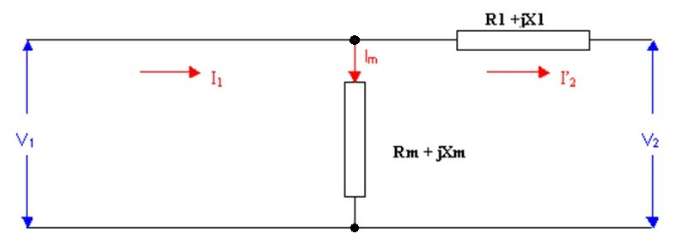
\includegraphics[width=0.7\textwidth]{equivalente_vacio.png}
    \captionsetup{labelformat=empty}
    \caption{Circuito equivalente para la condición de vacío.}
\end{figure}

\subsection{Prueba de cortocircuito}
Esta prueba se realiza a voltaje reducido, hasta que circule una corriente nominal por el circuito. En este caso no se toma la rama de magnetización, esto es debido a que solo se requiere un pequeño voltaje para obtener las corrientes nominales en los embobinados debido a que dichas impedancias son limitadas por la impedancia de dispersión de los embobinados, por lo tanto, la densidad de flujo en el núcleo será pequeña en la prueba de cortocircuito, las pérdidas en el núcleo y la corriente de magnetización será todavía más pequeña. La tensión reducida Vcc, llamada frecuentemente tensión de impedancia, se soluciona para que la corriente de cortocircuito Icc no ocasione daño en los enrollamientos. Se escoge usualmente Icc como la corriente de plena carga. Usualmente esta prueba se hace por el lado de alto voltaje.
\begin{figure}[H]
    \centering
    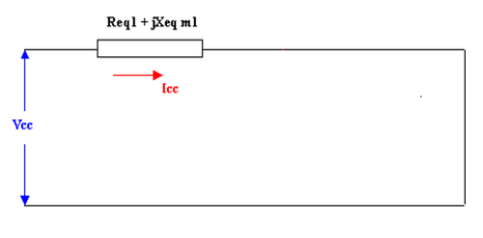
\includegraphics[width=0.7\textwidth]{equivalente_corto.png}
    \captionsetup{labelformat=empty}
    \caption{Circuito equivalente para la condición de cortocircuito.}
\end{figure}

\section{Cuestionario}
\begin{enumerate}
    \item Incluir en el informe los datos tomados en las experiencias realizadas.\\
    Datos de la prueba en vacío\cite{labo}:
    \begin{center}
        \begin{tabular}{ |c|c|c|c|c|c|c|c| } 
            \hline
            a & $V_{1}(V)$ & $I_{0}(A)$ & $P(W)$ & $V_{2}(V)$ & $FP(\%)$ & $S(VA)$ \\
            \hline
            1.7113 & 20.69 & 0.014 & 0.02 & 12.09 & 6.90 & 0.28966 \\ 
            1.7088 & 30.57 & 0.018 & 0.11 & 17.89 & 19.99 & 0.55026 \\ 
            1.7057 & 39.81 & 0.022 & 0.24 & 23.34 & 27.40 & 0.87582 \\ 
            1.7005 & 51.15 & 0.026 & 0.44 & 30.08 & 33.09 & 1.3299 \\ 
            1.6982 & 60.10 & 0.030 & 0.72 & 35.39 & 39.93 & 1.803 \\ 
            1.6970 & 70.80 & 0.035 & 1.05 & 41.72 & 42.37 & 2.478 \\ 
            1.6966 & 81.20 & 0.039 & 1.38 & 47.86 & 43.58 & 3.1668 \\ 
            1.6956 & 90.56 & 0.044 & 1.83 & 53.41 & 45.93 & 3.98464 \\ 
            1.6951 & 100.81 & 0.050 & 2.51 & 59.47 & 49.80 & 5.0405 \\ 
            1.6803 & 112.18 & 0.058 & 3.35 & 66.76 & 51.49 & 6.50644 \\ 
            \hline
        \end{tabular}
    \end{center}
    
    Datos de la prueba en corto circuito:
    \begin{center}
        \begin{tabular}{ |c|c|c|c|c|c|c|c| } 
            \hline
            $V_{1cc}(V)$ & $I_{1cc}(A)$ & $P_{cc}(W)$ & $FP(\%)$ & $S(VA)$ \\
            \hline
            2.095 & 1.000 & 1.976 & 94.30 & 2.095 \\ 
            2.400 & 1.250 & 2.840 & 94.67 & 3.000 \\ 
            3.280 & 1.720 & 5.366 & 95.12 & 5.642 \\ 
            4.200 & 2.220 & 8.898 & 95.43 & 9.324 \\ 
            4.828 & 2.530 & 11.701 & 95.79 & 12.215 \\ 
            5.550 & 2.920 & 15.577 & 96.12 & 16.206 \\ 
            6.620 & 3.470 & 22.144 & 96.40 & 22.971 \\ 
            7.500 & 3.940 & 28.634 & 96.90 & 29.550 \\ 
            8.14 & 4.280 & 34.003 & 97.60 & 34.839 \\ 
            \hline
        \end{tabular}
    \end{center}
    
    Datos de la prueba con carga
    \begin{center}
        \begin{tabular}{ |c|c|c|c|c|c|c|c| } 
            \hline
            $V_{1}(V)$ & $I_{1}(A)$ & $I_{2}(A)$ & $P(W)$ & $R_{p}:$ Resistencia Ensayada \\
            \hline
            220 & 2.320 & 4.000 & 466.56 & 29.46 \\ 
            220 & 1.760 & 3.000 & 350.2 & 39.5 \\ 
            220 & 1.200 & 2.000 & 233.6 & 59.75 \\ 
            220 & 0.640 & 1.000 & 114.84 & 120.88 \\ 
            \hline
        \end{tabular}
    \end{center}
    
    \item Del ensayo de vacío trazar las curvas de factor de potencia $cos\theta_{0}(\%)$, potencia consumida $P_{0}(W)$ y corriente en vacío $I_{0}(A)$ como funciones de la tensión de alimentación, asimismo graficar la curva relación de transformación.
    \begin{figure}[H]
    \centering
        \begin{minipage}{.5\textwidth}
          \centering
          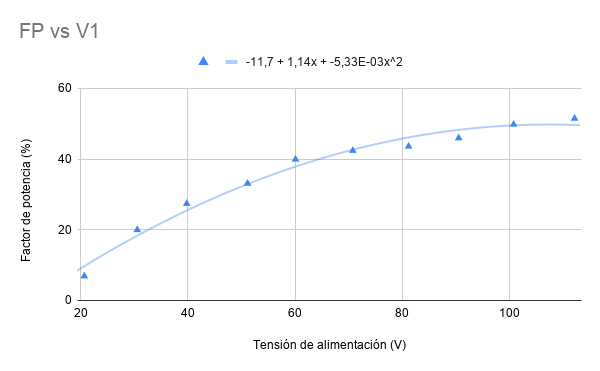
\includegraphics[width=.95\linewidth]{FPvsV1.png}
          \captionsetup{labelformat=empty}
          \captionof{figure}{Factor de Potencia vs Tensión de entrada.}
        \end{minipage}%
        \begin{minipage}{.5\textwidth}
          \centering
          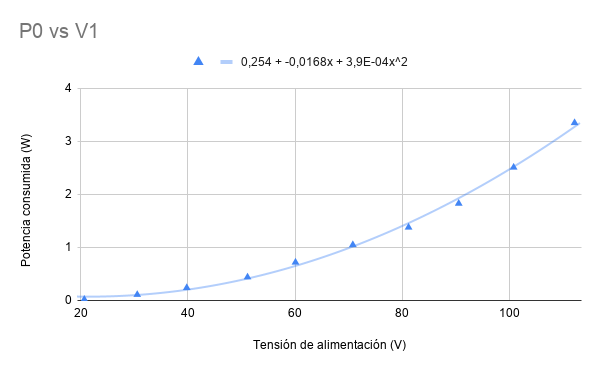
\includegraphics[width=.95\linewidth]{P0vsV1.png}
          \captionsetup{labelformat=empty}
          \captionof{figure}{Potencia consumida vs Tensión de entrada.}
        \end{minipage}
    \end{figure}
    
    \begin{figure}[H]
    \centering
        \begin{minipage}{.5\textwidth}
          \centering
          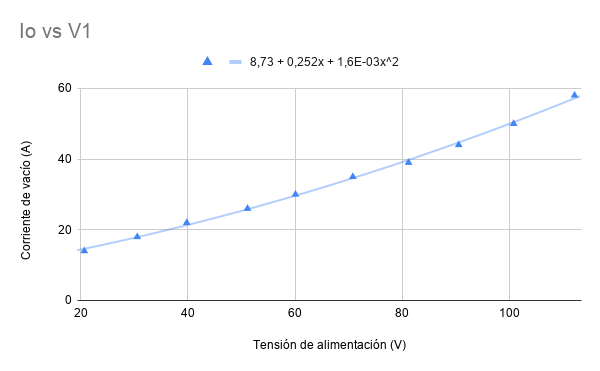
\includegraphics[width=.95\linewidth]{IovsV1.png}
          \captionsetup{labelformat=empty}
          \captionof{figure}{Corriente de vacío vs Tensión de entrada.}
        \end{minipage}%
        \begin{minipage}{.5\textwidth}
          \centering
          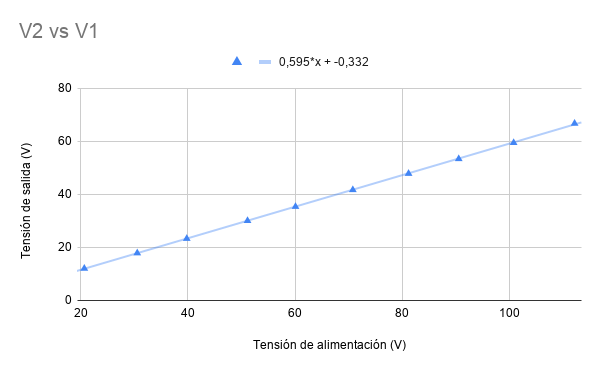
\includegraphics[width=1.0\linewidth]{V2vsV1.png}
          \captionsetup{labelformat=empty}
          \captionof{figure}{Relación de transformación.}
        \end{minipage}
    \end{figure}
    
    \item Del ensayo de cortocircuito graficar a partir de las lecturas la potencia consumida $P_{cc}(W)$, la tensión de impedancia $V_{cc}(V)$ y el factor de potencia de cortocircuito $cos\theta_{cc}(\%)$ como funciones de la corriente de cortocircuito $I_{cc}(A)$
    \begin{figure}[H]
    \centering
        \begin{minipage}{.5\textwidth}
          \centering
          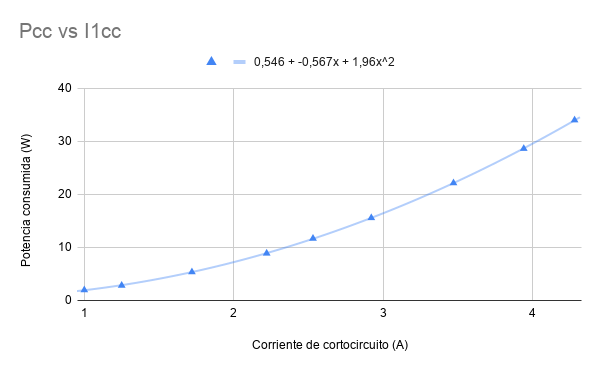
\includegraphics[width=1.0\linewidth]{PccvsI1cc.png}
          \captionsetup{labelformat=empty}
          \captionof{figure}{Potencia consumida vs Corriente de cortocircuito.}
        \end{minipage}%
        \begin{minipage}{.5\textwidth}
          \centering
          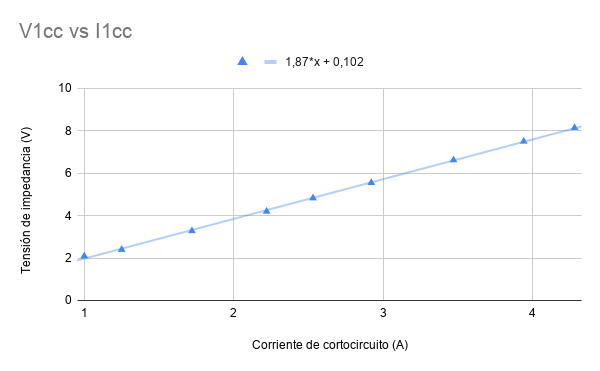
\includegraphics[width=1.0\linewidth]{V1ccvsI1cc.png}
          \captionsetup{labelformat=empty}
          \captionof{figure}{Tension de impedancia vs Corriente de cortocircuito.}
        \end{minipage}
    \end{figure}
    
    \begin{figure}[H]
    \centering
    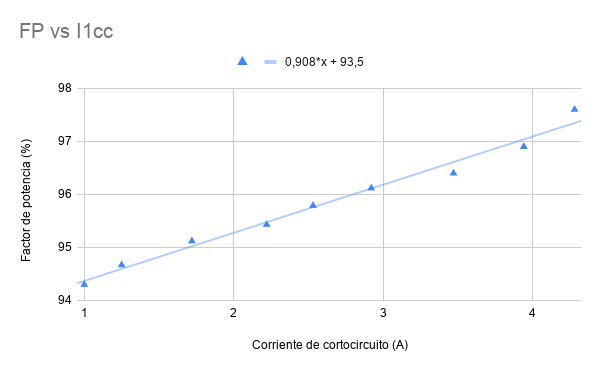
\includegraphics[width=0.6\textwidth]{FPvsI1cc.png}
    \captionsetup{labelformat=empty}
    \caption{Factor de potencia vs Corriente de cortocircuito.}
    \end{figure}
    
    \item Utilizando los datos de las dos primeras pruebas hallar el circuito equivalente exacto del transformador para condiciones nominales.\\
    Con los datos obtenidos, obtenemos la corriente de vacío y potencia respectiva para el voltaje nominal del primario V=110.
    \[V_{1}=110V ,I_{1}=0.056, P_{0}=3.17W\]
    De la prueba de vacío:
    \[g_{2}=\frac{P_{Fe}}{V_{0}^2}\]
    Las pérdidas del fierro son las mismas que las pérdidas obtenidas en el ensayo de vacío.
    \[g_{1}=\frac{3.17}{110^2}=261.983x10^{-8} mho\]
    También:
    \[b_{1}=\left(y_{0}^2-g_{1}^2\right)^{\frac{1}{2}}=\left(\left(\frac{I_{0}}{V_{0}}\right)^2-g_{1}^2\right)^{\frac{1}{2}}\]
    \[I_{0}=0.056A,V_{0}=110V\]
    Reemplazando se obtiene:
    \[b_{1}=436.507x10^{−6}mho\]
    Para la prueba de corto circuito interpolando los valores para la corriente nominal de $4A$:
    \[V_{cc}=8.04V,I_{cc}=4.00A,P_{cu}=31.16W\]
    \[R_{eq}=P_{cu}/I_{cc}^2=1.9475\Omega\]
    \[x_{eq}=\sqrt{Z_{eq}^2−R_{eq}^2}=\sqrt{\left(\frac{V_{cc}}{I_{cc}}\right)^2−R_{eq}^2}\]
    \[x_{eq}=0.497\Omega\]
    El circuito equivalente reducido al primario quedaría:
    \begin{figure}[H]
    \centering
    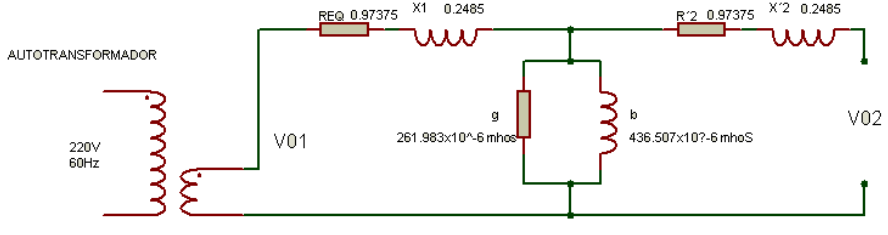
\includegraphics[width=0.7\textwidth]{lab_circuito.png}
    \captionsetup{labelformat=empty}
    \caption{\label{pi_} Circuito equivalente.}
    \end{figure}
    
    \item Con el circuito equivalente aproximado trazar el diagrama fasorial del transformador, es decir, $V_{a}$ vs $I_{a}$
    \begin{figure}[H]
    \centering
    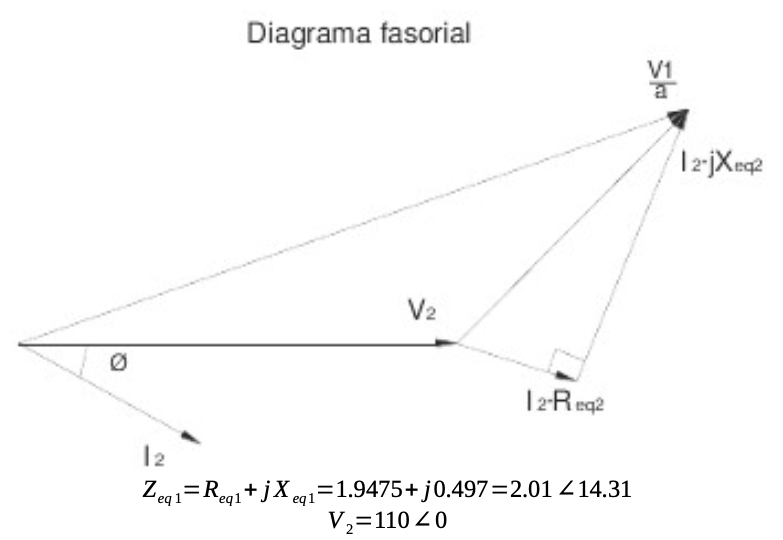
\includegraphics[width=0.6\textwidth]{fasorial.png}
    \captionsetup{labelformat=empty}
    \caption{\label{pi__} Diagrama fasorial.}
    \end{figure}
    
    \item Con los datos del ensayo con carga a factor de potencia 1, graficar la curva $V_{a}$ vs $I_{a}$ ,y compararlo con el gráfico encontrado en 4, explicar las diferencias.
    Sabemos que:
    \[V_{a}=E_{2}−Z_{eq2}I_{2}\]
    \begin{figure}[H]
    \centering
    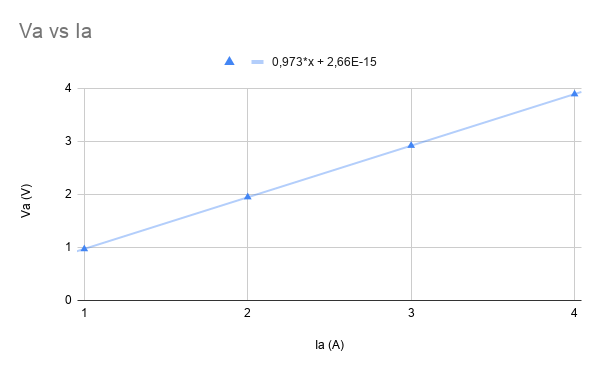
\includegraphics[width=0.7\textwidth]{VavsIa.png}
    \captionsetup{labelformat=empty}
    \caption{\label{pi___} Curva Va vs Ia.}
    \end{figure}
    
    \item Para las diversas cargas determinar la caída de tensión interna $\mu$ en \% según la expresión:
    \[\mu(\%)=\frac{V_{o2}-V_{2}}{V_{o2}}x100\]
    \begin{center}
        \begin{tabular}{ |c|c|c|c|c|c|c|c| } 
            \hline
            $E_{2}(V)$ & $V_{2}$ & $V_{a}(A)$ & $\mu(\%)$ \\
            \hline
            125.7 & 121.81 & 3.89 & 3.193\\
            126.01 & 123.09 & 2.92 & 2.372\\
            126.32 & 124.37 & 1.95 & 1.568\\
            126.63 & 125.66 & 0.97 & 0.772\\
            \hline
        \end{tabular}
    \end{center}
    
    \item Calcular la regulación de tensión para carga nominal con $Cos\phi=0.8$ capacitivo. Asimismo calcular la eficiencia del transformador para estas condiciones:
    \[\eta=\frac{V_{AN}I_{AN}cos\theta}{V_{2N}I_{2N}cos\theta+P_{0}+P_{L}(75ºC)}\]
    \[r=\left[\frac{I_{n2}\left(R_{2}cos\theta+X_{2}sen\theta\right)}{V_{2n}}+\frac{1}{2}\left(\frac{I_{2n}\left(X_{2}cos\theta-R_{2}sen\theta\right)}{V_{2n}}\right)^2\right]100\]
    \[V_{2n}=110V;I_{2n}=4A;R_{2}=0.2434;X_{2}=0.062125\]
    Reemplazando en la ecuación la regulación de tensión es:
    \[r=0.89\]
    La eficiencia del transformador:
    \[\eta=90.82(\%)\]
    
    \item Comparar las pérdidas en el cobre $I_{1N}^2R_{T}(W)$ con las pérdidas de carga $P_{L}(75ºC)$ dada por la expresión:
    \begin{equation}
    \label{eq:campo}
        P_{L}(75ºC)=I_{1N}^2R_{1}+\frac{235+75}{235+t}+\left(P_{cc}(t)-I_{1N}^2R_{1}\right)\frac{235+t}{235+75}
    \end{equation}
    Donde:\\
    \hspace*{3em}
    \begin{tabular}{rl}
        $I_{1N}$:& Corriente nominal en el primario. \\
        $R_{t}$:& Resistencia equivalente en el arrollamiento primario a $tºC=R_{1t}+a^2R_{2t}$. \\
    \end{tabular}
    Las pérdidas en el cobre han sido halladas en el ensayo de cortocircuito.
    \[I_{1n}^2R_{t}=31.16W\]
    Con los datos hallados en la experiencia e interpolando tenemos los siguientes datos Para nuestra experiencia usaremos: $T=23C$
    \[I_{1n}=4A;P_{cc}=31.16W;R_{1}=0.9737\Omega;I_{2n}^2R_{1}=15.58W\]
    Reemplazamos en la Ec.~\eqref{eq:campo}:
    \[P_{L}=45.3281W\]
    Observamos que las pérdidas en el cobre $I_{1n}^2R_{t}$ y las perdidas en la carga $P_{l}$ a $75C$ son valores cercanos.
\end{enumerate}

